%%%%%%%%%%%%%%%%%%%%%%%%%%%%%%%%%%%%%%%%%
% Homework Assignment Article
% LaTeX Template
% Version 1.3.1 (ECL) (08/08/17)
%
% This template has been downloaded from:
% Overleaf
%
% Original author:
% Victor Zimmermann (zimmermann@cl.uni-heidelberg.de)
%
% License:
% CC BY-SA 4.0 (https://creativecommons.org/licenses/by-sa/4.0/)
%
%%%%%%%%%%%%%%%%%%%%%%%%%%%%%%%%%%%%%%%%%

%----------------------------------------------------------------------------------------

\documentclass[a4paper]{article} % Uses article class in A4 format

%----------------------------------------------------------------------------------------
%	FORMATTING
%----------------------------------------------------------------------------------------

\addtolength{\hoffset}{-2.25cm}
\addtolength{\textwidth}{4.5cm}
\addtolength{\voffset}{-3.25cm}
\addtolength{\textheight}{5cm}
\setlength{\parskip}{6pt}
\setlength{\parindent}{0in}

%----------------------------------------------------------------------------------------
%	PACKAGES AND OTHER DOCUMENT CONFIGURATIONS
%----------------------------------------------------------------------------------------

\usepackage{blindtext} % Package to generate dummy text
% \usepackage[style=numeric,sorting=none]{biblatex}
\usepackage{charter} % Use the Charter font
\usepackage[utf8]{inputenc} % Use UTF-8 encoding
\usepackage{microtype} % Slightly tweak font spacing for aesthetics

\usepackage[english]{babel} % Language hyphenation and typographical rules

\usepackage{amsthm, amsmath, amssymb} % Mathematical typesetting
\usepackage{float} % Improved interface for floating objects
\usepackage[final, colorlinks = true, 
            linkcolor = black, 
            citecolor = black]{hyperref} % For hyperlinks in the PDF
\usepackage{graphicx, multicol} % Enhanced support for graphics
\usepackage{xcolor} % Driver-independent color extensions
\usepackage{marvosym, wasysym} % More symbols
\usepackage{rotating} % Rotation tools
\usepackage{censor} % Facilities for controlling restricted text
\usepackage{listings, style/lstlisting} % Environment for non-formatted code, !uses style file!
\usepackage{pseudocode} % Environment for specifying algorithms in a natural way
\usepackage{style/avm} % Environment for f-structures, !uses style file!
\usepackage{booktabs} % Enhances quality of tables

\usepackage{tikz-qtree} % Easy tree drawing tool
\tikzset{every tree node/.style={align=center,anchor=north},
         level distance=2cm} % Configuration for q-trees
\usepackage{style/btree} % Configuration for b-trees and b+-trees, !uses style file!

% \usepackage[backend=biber,style=numeric,
            % sorting=nyt]{biblatex} % Complete reimplementation of bibliographic facilities
% \addbibresource{ecl.bib}
\usepackage{csquotes} % Context sensitive quotation facilities

\usepackage[yyyymmdd]{datetime} % Uses YEAR-MONTH-DAY format for dates
\renewcommand{\dateseparator}{-} % Sets dateseparator to '-'

\usepackage{fancyhdr} % Headers and footers
\pagestyle{fancy} % All pages have headers and footers
\fancyhead{}\renewcommand{\headrulewidth}{0pt} % Blank out the default header
\fancyfoot[L]{School of Computing, Macquarie University} % Custom footer text
\fancyfoot[C]{} % Custom footer text
\fancyfoot[R]{\thepage} % Custom footer text

\usepackage{comment}
\newcommand{\note}[1]{\marginpar{\scriptsize \textcolor{red}{#1}}} % Enables comments in red on margin

%----------------------------------------------------------------------------------------

\begin{document}

%----------------------------------------------------------------------------------------
%	TITLE SECTION
%----------------------------------------------------------------------------------------

\title{COMP3100 project report} % Article title
\fancyhead[C]{}
\hrule \medskip % Upper rule
\begin{minipage}{1\textwidth} % Center of title section
\centering 
\large % Title text size
Project report: Stage 1\\ % Assignment title and number
COMP3100 Distributed Systems, S2, 2022\\
\normalsize % Subtitle text size
SID: 4481 6936, Name: Jacob Temperley
%%%%\\ % Assignment subtitle
\end{minipage}
\medskip\hrule % Lower rule
\bigskip

%----------------------------------------------------------------------------------------
%	ARTICLE CONTENTS
%----------------------------------------------------------------------------------------
\section{Introduction}
Distributed systems inherently require that large tasks be broken up into smaller, more manageable tasks. Examples of tasks that distributed systems solve includes ‘provide access to a website’ which may be divided up between many servers and many web requests, or ‘render this image’ which may be divided up into fragments of an image and sent to parallel processors on a GPU. In all these examples the distributed system looks externally like a single coherent system but is really a carefully coordinated network of parallel systems; the problem of coordinating such systems is often referred to as ‘scheduling’.\par
On a multi-core computer for example, the cores are managed by a thread-scheduler which takes discrete program (or threads in a program) and distributes them over the available cores making sure all programs get a fair share of the available processing power. A similar process occurs in web server management where a single server is not sufficient to serve all clients, so a load balancer (another scheduler) is used to spread requests over many servers.\par
The goal of this project is to implement a simple scheduler which will assign jobs to servers. The scheduler will utilise a Largest Round Robin (LRR) algorithm to spread jobs over the most powerful servers available. The algorithm is simple: find the server type that has the highest number of cores and assign sequential jobs by rotating through servers of that type. 


\section{System overview}
\label{sec:section2}

The scheduling system is made up of two parts: the scheduler (referred to as the client client) and the simulated servers (referred to as server). The java client is the portion of the system we have modified to use the LRR algorithm and initiates the work done on the servers. Our client goes through three major stages (which are outlined in figure 1), \begin{enumerate}
    \item Initiation, where the client connects with the server and collects simulated server information.
    \item The algorithm loop, which applies the algorithm to the server information, jobs, and makes scheduling decisions.
    \item Termination, where the client notifies the server it is disconnecting.
\end{enumerate}
\begin{figure}
    \centering
    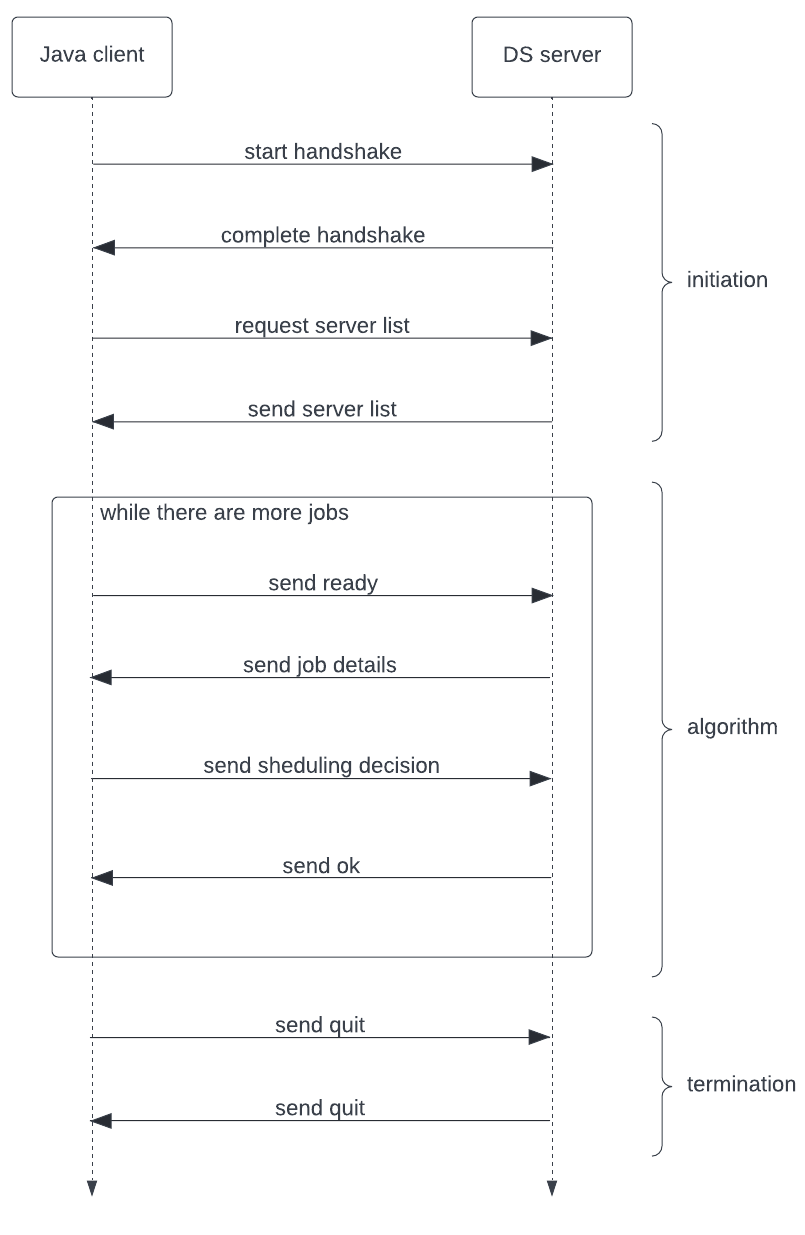
\includegraphics{over.png}
    \caption{The high-level lifecycle of the interaction between the server and client}
    \label{fig:overview}
\end{figure}


\section{Design}
\subsection{Design paradigm/philosophy}
The design paradigm underlying this project was, almost by necessity, object-oriented (as opposed to functional or procedural) because of Java’s inherently object-oriented nature. We could have taken a c-like procedural approach, which was the style of the early iterations for this project, but Java’s lack of function pointers (instead using lambdas) means that refactoring this style is painful at best. Instead the refactoring included reworking the program into a neatly packaged set of 3 classes: Client, Scheduler (an interface), and LRR (implementing Scheduler).\par
This paradigm supports the main philosophical pillars considered when building this project which are common to many programmers, namely, reusability, the principle of least knowledge, and readability. 
\begin{itemize}
    \item Reusability: the classes should not be so specific or coupled to the use case that it cannot be reused in other programs, or for other purposes.
    \item Readability: other programmers (who are not specialised in java) should be able to read the code and derive at least a rudimentary knowledge of the structure and function.
    \item Principle of least knowledge: a programmer should not need to know the inner workings of the classes to use them, i.e. we only need to know how to use them, not how they work. 
\end{itemize}

\subsection{Considerations and constraints}
The reasons for these specific philosophical pillars really comes down to being lazy (as many thing in IT do) because we know that there will be more algorithms to implement in the future, and we don’t want to re-learn how the system works (we will inevitably forget the fine details) or re-write code that has the same purpose. With this in mind, we want to be able to write a new scheduling algorithm and insert it back into the program without any extra modifications. 

\subsection{Functionality}
The functionality of the client and server can be described by a simple request-reply schema, even if the message sent by the client is not semantically a ‘request’ (OK message for example) the server will always make a reply.\par
The client has the responsibilities of,
\begin{itemize}
    \item Initiating the connection
    \item Initiating the handshake
    \item Requesting server/job information
    \item Scheduling jobs
    \item Terminating the connection
\end{itemize}

The server has the responsibilities of,
\begin{itemize}
    \item Loading/managing job and server information
    \item Replying to incoming messages
    \item Applying scheduling decisions
    \item Simulating job processing/completion by server 
\end{itemize}

\section{Implementation}
\subsection{Design pattern}
Starting from the largest scale implementation details, we have one main object-oriented pattern, a strategy pattern. This is where the scheduling algorithm is encapsulated into its own class and implements the Scheduler interface. The client has a Scheduler but doesn’t need to know the exact implementation of it, meaning we can define a new Scheduler that uses a different algorithm later and insert it into the client. For now, we only have one algorithm which is the Largest Round Robin (LRR). This setup of composition and implementation is shown in figure 2 where the black diamond indicates the composition relationship between Client and Scheduler, and the implementing relationship is indicated by the dotted arrow between Scheduler and LRR.

\begin{figure}
    \centering
    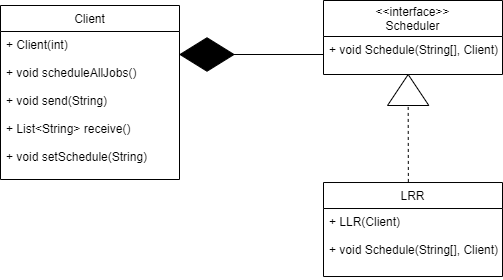
\includegraphics{class.png}
    \caption{The class diagram for the client portion of our distributed systems scheduling algorithm.}
    \label{fig:class}
\end{figure}

\subsection{Class details}

Diving a little deeper into the client code, it’s all written in Java and uses some of the native java libraries. The most important of these libraries is java.net of which we use the Socket\cite{socket} class. The Socket class encapsulates the networking concept of an IP address combined with a port which is used to direct packets to another program. In our case the other program is on the local machine which means the IP address is not necessary, but the socket still requires a port to properly address the destination.\par
We also require java.io, of which we used two important classes: DataOutputSream\cite{out} and BufferedReader\cite{read}. Both of these classes are very similar, they wrap data streams to and from the Socket so we can send and receive messages from the server program. Our Client class takes this a step further and wraps the Socket, DataOutputSream, BufferedReader, and Scheduler into a single class which manages the job scheduling for the server.
\subsubsection{Client}
The Client is broken up into 3 crucial parts: the constructor Client(), receive(), and send(). The constructor takes a port number which sets up the socket, streams, and does the handshake protocol with the server. The send() function just hides the details of the DataOutputStream, you pass send() a message, which is processed and sent. The receive() function simplifies the processing of message from the server, which may by multiple lines of response (from a GETS for example) or a job completion message (which is recursively discarded). Finally the scheduleAllJobs() is just a function which loops through send(), receive() and schedule() until all jobs are complete.\par
\subsubsection{LRR}
Finally the LRR scheduler has only 2 functions, the constructor and schedule(). The constructor sets up LRR with all the data it needs to make scheduling decisions (this may not be the case for future algorithms), importantly it gets the server list and determines the largest server type. Schedule() then rotates scheduling through all of the largest servers, one by one.
All of the classes also use standard java.util List and ArrayList to manage variable length lists where necessary.


\subsection{Github link}
\url{https://github.com/jetemperley/COMP3100ass}
\bibliographystyle{plain}
\bibliography{comp3100project}
\end{document}
